% Options for packages loaded elsewhere
\PassOptionsToPackage{unicode}{hyperref}
\PassOptionsToPackage{hyphens}{url}
%
\documentclass[
]{article}
\usepackage{lmodern}
\usepackage{amssymb,amsmath}
\usepackage{ifxetex,ifluatex}
\ifnum 0\ifxetex 1\fi\ifluatex 1\fi=0 % if pdftex
  \usepackage[T1]{fontenc}
  \usepackage[utf8]{inputenc}
  \usepackage{textcomp} % provide euro and other symbols
\else % if luatex or xetex
  \usepackage{unicode-math}
  \defaultfontfeatures{Scale=MatchLowercase}
  \defaultfontfeatures[\rmfamily]{Ligatures=TeX,Scale=1}
\fi
% Use upquote if available, for straight quotes in verbatim environments
\IfFileExists{upquote.sty}{\usepackage{upquote}}{}
\IfFileExists{microtype.sty}{% use microtype if available
  \usepackage[]{microtype}
  \UseMicrotypeSet[protrusion]{basicmath} % disable protrusion for tt fonts
}{}
\makeatletter
\@ifundefined{KOMAClassName}{% if non-KOMA class
  \IfFileExists{parskip.sty}{%
    \usepackage{parskip}
  }{% else
    \setlength{\parindent}{0pt}
    \setlength{\parskip}{6pt plus 2pt minus 1pt}}
}{% if KOMA class
  \KOMAoptions{parskip=half}}
\makeatother
\usepackage{xcolor}
\IfFileExists{xurl.sty}{\usepackage{xurl}}{} % add URL line breaks if available
\IfFileExists{bookmark.sty}{\usepackage{bookmark}}{\usepackage{hyperref}}
\hypersetup{
  pdftitle={Assignment2},
  pdfauthor={Haojin Li (Declan)},
  hidelinks,
  pdfcreator={LaTeX via pandoc}}
\urlstyle{same} % disable monospaced font for URLs
\usepackage[margin=1in]{geometry}
\usepackage{color}
\usepackage{fancyvrb}
\newcommand{\VerbBar}{|}
\newcommand{\VERB}{\Verb[commandchars=\\\{\}]}
\DefineVerbatimEnvironment{Highlighting}{Verbatim}{commandchars=\\\{\}}
% Add ',fontsize=\small' for more characters per line
\usepackage{framed}
\definecolor{shadecolor}{RGB}{248,248,248}
\newenvironment{Shaded}{\begin{snugshade}}{\end{snugshade}}
\newcommand{\AlertTok}[1]{\textcolor[rgb]{0.94,0.16,0.16}{#1}}
\newcommand{\AnnotationTok}[1]{\textcolor[rgb]{0.56,0.35,0.01}{\textbf{\textit{#1}}}}
\newcommand{\AttributeTok}[1]{\textcolor[rgb]{0.77,0.63,0.00}{#1}}
\newcommand{\BaseNTok}[1]{\textcolor[rgb]{0.00,0.00,0.81}{#1}}
\newcommand{\BuiltInTok}[1]{#1}
\newcommand{\CharTok}[1]{\textcolor[rgb]{0.31,0.60,0.02}{#1}}
\newcommand{\CommentTok}[1]{\textcolor[rgb]{0.56,0.35,0.01}{\textit{#1}}}
\newcommand{\CommentVarTok}[1]{\textcolor[rgb]{0.56,0.35,0.01}{\textbf{\textit{#1}}}}
\newcommand{\ConstantTok}[1]{\textcolor[rgb]{0.00,0.00,0.00}{#1}}
\newcommand{\ControlFlowTok}[1]{\textcolor[rgb]{0.13,0.29,0.53}{\textbf{#1}}}
\newcommand{\DataTypeTok}[1]{\textcolor[rgb]{0.13,0.29,0.53}{#1}}
\newcommand{\DecValTok}[1]{\textcolor[rgb]{0.00,0.00,0.81}{#1}}
\newcommand{\DocumentationTok}[1]{\textcolor[rgb]{0.56,0.35,0.01}{\textbf{\textit{#1}}}}
\newcommand{\ErrorTok}[1]{\textcolor[rgb]{0.64,0.00,0.00}{\textbf{#1}}}
\newcommand{\ExtensionTok}[1]{#1}
\newcommand{\FloatTok}[1]{\textcolor[rgb]{0.00,0.00,0.81}{#1}}
\newcommand{\FunctionTok}[1]{\textcolor[rgb]{0.00,0.00,0.00}{#1}}
\newcommand{\ImportTok}[1]{#1}
\newcommand{\InformationTok}[1]{\textcolor[rgb]{0.56,0.35,0.01}{\textbf{\textit{#1}}}}
\newcommand{\KeywordTok}[1]{\textcolor[rgb]{0.13,0.29,0.53}{\textbf{#1}}}
\newcommand{\NormalTok}[1]{#1}
\newcommand{\OperatorTok}[1]{\textcolor[rgb]{0.81,0.36,0.00}{\textbf{#1}}}
\newcommand{\OtherTok}[1]{\textcolor[rgb]{0.56,0.35,0.01}{#1}}
\newcommand{\PreprocessorTok}[1]{\textcolor[rgb]{0.56,0.35,0.01}{\textit{#1}}}
\newcommand{\RegionMarkerTok}[1]{#1}
\newcommand{\SpecialCharTok}[1]{\textcolor[rgb]{0.00,0.00,0.00}{#1}}
\newcommand{\SpecialStringTok}[1]{\textcolor[rgb]{0.31,0.60,0.02}{#1}}
\newcommand{\StringTok}[1]{\textcolor[rgb]{0.31,0.60,0.02}{#1}}
\newcommand{\VariableTok}[1]{\textcolor[rgb]{0.00,0.00,0.00}{#1}}
\newcommand{\VerbatimStringTok}[1]{\textcolor[rgb]{0.31,0.60,0.02}{#1}}
\newcommand{\WarningTok}[1]{\textcolor[rgb]{0.56,0.35,0.01}{\textbf{\textit{#1}}}}
\usepackage{graphicx,grffile}
\makeatletter
\def\maxwidth{\ifdim\Gin@nat@width>\linewidth\linewidth\else\Gin@nat@width\fi}
\def\maxheight{\ifdim\Gin@nat@height>\textheight\textheight\else\Gin@nat@height\fi}
\makeatother
% Scale images if necessary, so that they will not overflow the page
% margins by default, and it is still possible to overwrite the defaults
% using explicit options in \includegraphics[width, height, ...]{}
\setkeys{Gin}{width=\maxwidth,height=\maxheight,keepaspectratio}
% Set default figure placement to htbp
\makeatletter
\def\fps@figure{htbp}
\makeatother
\setlength{\emergencystretch}{3em} % prevent overfull lines
\providecommand{\tightlist}{%
  \setlength{\itemsep}{0pt}\setlength{\parskip}{0pt}}
\setcounter{secnumdepth}{-\maxdimen} % remove section numbering

\title{Assignment2}
\author{Haojin Li (Declan)}
\date{2020/7/23}

\begin{document}
\maketitle

{
\setcounter{tocdepth}{2}
\tableofcontents
}
\hypertarget{exercises}{%
\subsection{\# 3.2.4 Exercises}\label{exercises}}

\hypertarget{run-ggplotdata-mpg.-what-do-you-see}{%
\subsection{\texorpdfstring{1. Run \texttt{ggplot(data\ =\ mpg)}. What
do you
see?}{1. Run ggplot(data = mpg). What do you see?}}\label{run-ggplotdata-mpg.-what-do-you-see}}

\begin{Shaded}
\begin{Highlighting}[]
\KeywordTok{library}\NormalTok{(ggplot2)}
\KeywordTok{ggplot}\NormalTok{(}\DataTypeTok{data =}\NormalTok{ mpg)}
\end{Highlighting}
\end{Shaded}


\includegraphics{Assignment-2_files/figure-latex/unnamed-chunk-1-1.pdf}
I see nothing\ldots{}

\hypertarget{how-many-rows-are-in-mpg-how-many-columns}{%
\subsection{\texorpdfstring{2. How many rows are in \texttt{mpg}? How
many
columns?}{2. How many rows are in mpg? How many columns?}}\label{how-many-rows-are-in-mpg-how-many-columns}}

\begin{Shaded}
\begin{Highlighting}[]
\KeywordTok{dim}\NormalTok{(mpg)}
\end{Highlighting}
\end{Shaded}

\begin{verbatim}
## [1] 234  11
\end{verbatim}

\hypertarget{what-does-the-drv-variable-describe-read-the-help-for-mpg-to-find-out.}{%
\subsection{\texorpdfstring{3. What does the \texttt{drv} variable
describe? Read the help for \texttt{?mpg} to find
out.}{3. What does the drv variable describe? Read the help for ?mpg to find out.}}\label{what-does-the-drv-variable-describe-read-the-help-for-mpg-to-find-out.}}

\begin{Shaded}
\begin{Highlighting}[]
\NormalTok{?}\KeywordTok{mpg}\NormalTok{()}
\end{Highlighting}
\end{Shaded}

\begin{verbatim}
## starting httpd help server ... done
\end{verbatim}

\begin{Shaded}
\begin{Highlighting}[]
\CommentTok{# `drv` is the type of drive train, where `f = front-wheel drive`, `r = rear wheel drive`, `4 = 4wd`}
\end{Highlighting}
\end{Shaded}

\hypertarget{make-a-scatterplot-of-hwy-vs-cyl.}{%
\subsection{\texorpdfstring{4. Make a scatterplot of \texttt{hwy} vs
\texttt{cyl}.}{4. Make a scatterplot of hwy vs cyl.}}\label{make-a-scatterplot-of-hwy-vs-cyl.}}

\begin{Shaded}
\begin{Highlighting}[]
\KeywordTok{library}\NormalTok{(ggplot2)}
\KeywordTok{ggplot}\NormalTok{(mpg, }\KeywordTok{aes}\NormalTok{(hwy, cyl)) }\OperatorTok{+}\StringTok{ }\KeywordTok{geom_point}\NormalTok{()}
\end{Highlighting}
\end{Shaded}

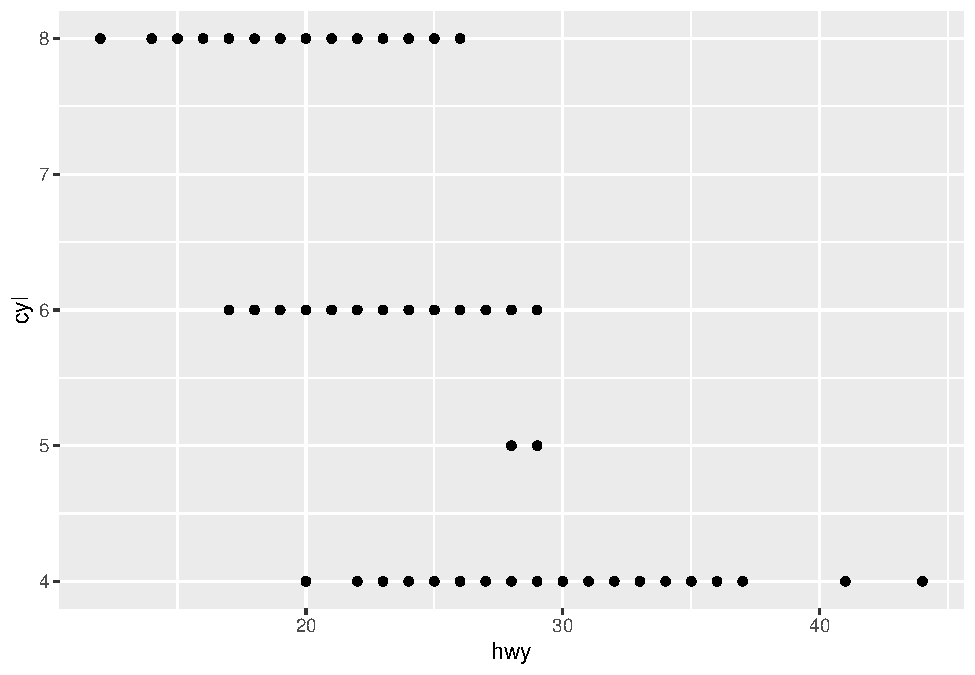
\includegraphics{Assignment-2_files/figure-latex/unnamed-chunk-4-1.pdf}

\begin{Shaded}
\begin{Highlighting}[]
\CommentTok{# plot(mpg$hwy, mpg$cyl, xlab="hwy", ylab="cyl")}
\end{Highlighting}
\end{Shaded}

\hypertarget{what-happens-if-you-make-a-scatterplot-of-class-vs-drv-why-is-the-plot-not-useful}{%
\subsubsection{\texorpdfstring{5. What happens if you make a scatterplot
of \texttt{class} vs \texttt{drv}? Why is the plot not
useful?}{5. What happens if you make a scatterplot of class vs drv? Why is the plot not useful?}}\label{what-happens-if-you-make-a-scatterplot-of-class-vs-drv-why-is-the-plot-not-useful}}

\begin{Shaded}
\begin{Highlighting}[]
\KeywordTok{library}\NormalTok{(ggplot2)}
\KeywordTok{ggplot}\NormalTok{(mpg, }\KeywordTok{aes}\NormalTok{(class, drv)) }\OperatorTok{+}\StringTok{ }\KeywordTok{geom_point}\NormalTok{()}
\end{Highlighting}
\end{Shaded}

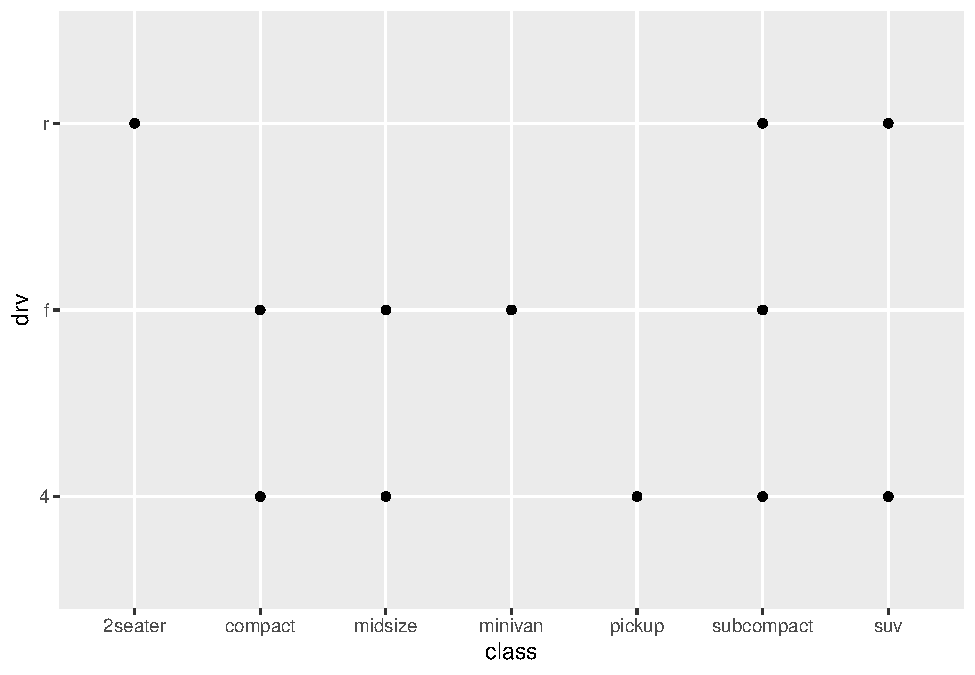
\includegraphics{Assignment-2_files/figure-latex/unnamed-chunk-5-1.pdf}

There's no correlation between \texttt{class} and \texttt{drv}.

\hypertarget{exercises-1}{%
\subsection{\# 3.3.1 Exercises}\label{exercises-1}}

\hypertarget{section}{%
\subsection{1}\label{section}}

\begin{Shaded}
\begin{Highlighting}[]
\KeywordTok{ggplot}\NormalTok{(}\DataTypeTok{data =}\NormalTok{ mpg) }\OperatorTok{+}\StringTok{ }
\StringTok{  }\KeywordTok{geom_point}\NormalTok{(}\DataTypeTok{mapping =} \KeywordTok{aes}\NormalTok{(}\DataTypeTok{x =}\NormalTok{ displ, }\DataTypeTok{y =}\NormalTok{ hwy), }\DataTypeTok{color =} \StringTok{"blue"}\NormalTok{)}
\end{Highlighting}
\end{Shaded}

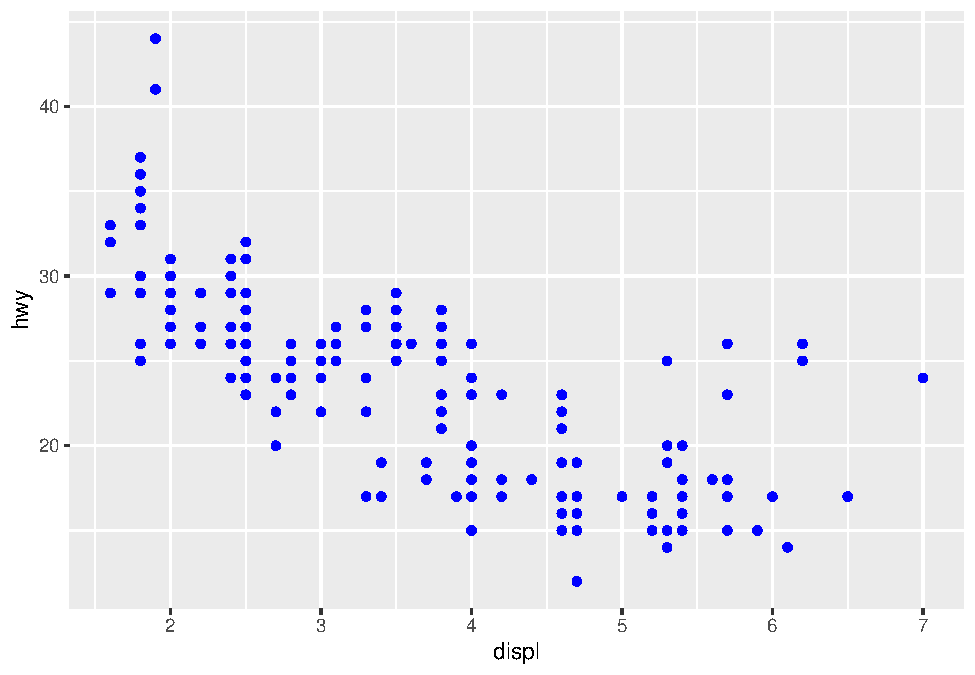
\includegraphics{Assignment-2_files/figure-latex/unnamed-chunk-6-1.pdf}

\hypertarget{section-1}{%
\subsection{2}\label{section-1}}

\begin{Shaded}
\begin{Highlighting}[]
\NormalTok{mpg}
\end{Highlighting}
\end{Shaded}

\begin{verbatim}
## # A tibble: 234 x 11
##    manufacturer model    displ  year   cyl trans   drv     cty   hwy fl    class
##    <chr>        <chr>    <dbl> <int> <int> <chr>   <chr> <int> <int> <chr> <chr>
##  1 audi         a4         1.8  1999     4 auto(l~ f        18    29 p     comp~
##  2 audi         a4         1.8  1999     4 manual~ f        21    29 p     comp~
##  3 audi         a4         2    2008     4 manual~ f        20    31 p     comp~
##  4 audi         a4         2    2008     4 auto(a~ f        21    30 p     comp~
##  5 audi         a4         2.8  1999     6 auto(l~ f        16    26 p     comp~
##  6 audi         a4         2.8  1999     6 manual~ f        18    26 p     comp~
##  7 audi         a4         3.1  2008     6 auto(a~ f        18    27 p     comp~
##  8 audi         a4 quat~   1.8  1999     4 manual~ 4        18    26 p     comp~
##  9 audi         a4 quat~   1.8  1999     4 auto(l~ 4        16    25 p     comp~
## 10 audi         a4 quat~   2    2008     4 manual~ 4        20    28 p     comp~
## # ... with 224 more rows
\end{verbatim}

\hypertarget{catagorical-variables}{%
\subsubsection{Catagorical Variables}\label{catagorical-variables}}

manufacturer model trans drv fl class

\hypertarget{continuous-variables}{%
\subsubsection{Continuous Variables}\label{continuous-variables}}

displ year cyl cty hwy

\hypertarget{section-2}{%
\subsection{3}\label{section-2}}

\begin{Shaded}
\begin{Highlighting}[]
\KeywordTok{ggplot}\NormalTok{(mpg, }\KeywordTok{aes}\NormalTok{(}\DataTypeTok{x =}\NormalTok{ displ, }\DataTypeTok{y =}\NormalTok{ hwy, }\DataTypeTok{colour =}\NormalTok{ cty)) }\OperatorTok{+}
\StringTok{  }\KeywordTok{geom_point}\NormalTok{()}
\end{Highlighting}
\end{Shaded}

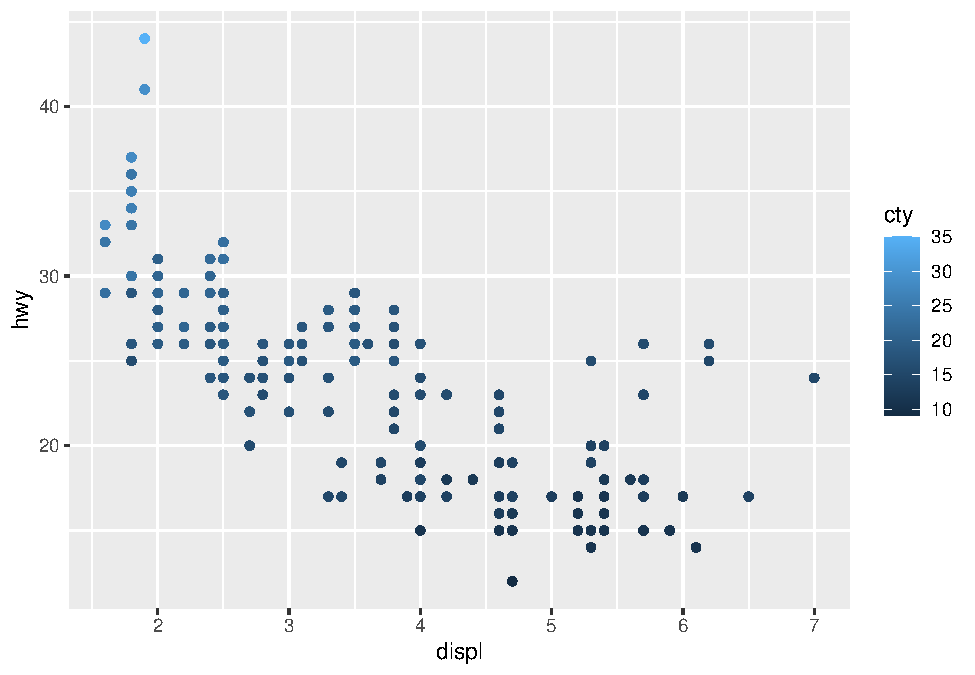
\includegraphics{Assignment-2_files/figure-latex/unnamed-chunk-8-1.pdf}

\begin{Shaded}
\begin{Highlighting}[]
\KeywordTok{ggplot}\NormalTok{(mpg, }\KeywordTok{aes}\NormalTok{(}\DataTypeTok{x =}\NormalTok{ displ, }\DataTypeTok{y =}\NormalTok{ hwy, }\DataTypeTok{size =}\NormalTok{ cty)) }\OperatorTok{+}
\StringTok{  }\KeywordTok{geom_point}\NormalTok{()}
\end{Highlighting}
\end{Shaded}

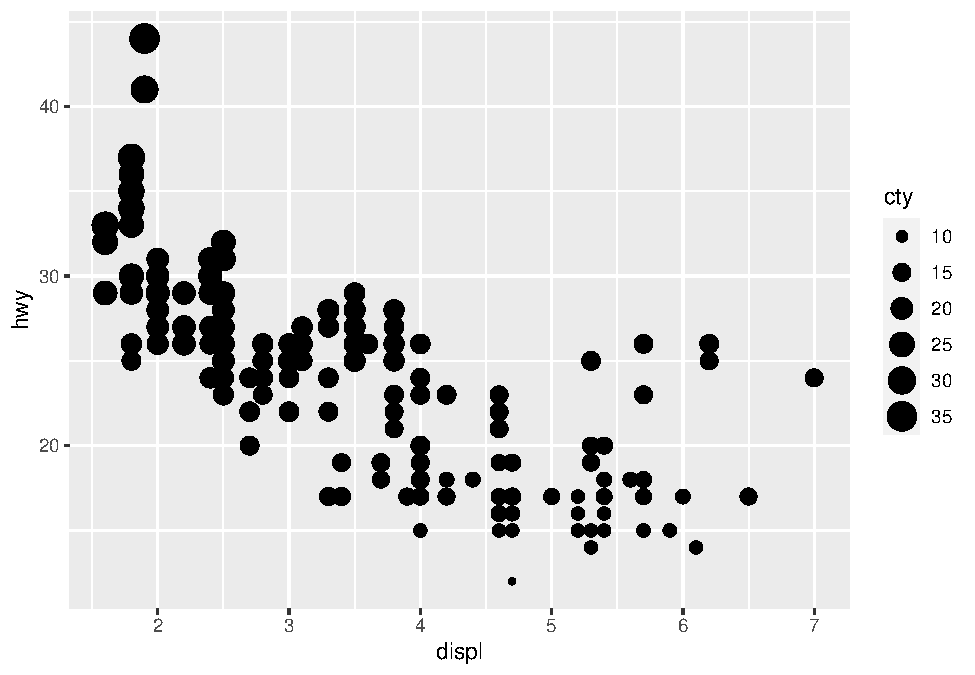
\includegraphics{Assignment-2_files/figure-latex/unnamed-chunk-9-1.pdf}

\end{document}
